\documentclass{cmc}
\usepackage{makecell}
\begin{document}

\pagestyle{fancy}
\lhead{\textit{\textbf{Computational Motor Control, Spring 2019} \\
    Webots exercise, Lab 9, GRADED}} \rhead{Bonnesoeur Maxime\\ Gautier Maxime\\ Furrer Stanislas}

\section*{Student names: Bonnesoeur Maxime, Gautier Maxime, \\ Furrer Stanislas}

\textit{Instructions: Update this file (or recreate a similar one, e.g.\ in
  Word) to prepare your answers to the questions. Feel free to add text,
  equations and figures as needed. Hand-written notes, e.g.\ for the development
  of equations, can also be included e.g.\ as pictures (from your cell phone or
  from a scanner).  \textbf{\corr{This lab is graded.}} and needs to be
  submitted before the \textbf{\corr{Deadline : Wednesday 15-05-2019
      Midnight. You only need to submit one final report for all of the
      following exercises combined henceforth.}} Please submit both the source
  file (*.doc/*.tex) and a pdf of your document, as well as all the used and
  updated Python functions in a single zipped file called
  \corr{final\_report\_name1\_name2\_name3.zip} where name\# are the team
  member’s last names.  \corr{Please submit only one report per team!}}
\\

\corr{\textit{NOTE : }}The following exercises on Salamandra robotica are based
on the research of \cite{Crespi2013}, \cite{Karakasiliotis2013} and
\cite{ijspeert2007swimming}.

\section*{Swimming with Salamandra robotica – CPG Model}
\label{sec:exploring-swimming}

In this exercise you will control a salamander-like robot Salamandra
robotica for which you will use Python and the dynamics simulator
Webots. Now you have an opportunity to use what you’ve learned until
now to make the robot swim (and eventually walk). In order to do this,
you should implement a CPG based swimming controller, similarly to the
architecture shown in Figure~\ref{fig:controller-model}.

In the folder Webots you will find sub folders containing the simulated
world file and Python codes describing the controller.
\corr{\textbf{\textit{NOTE : }}Do not change the relative positions of
  files within those folders.}

\begin{figure}[h]
  \centering
  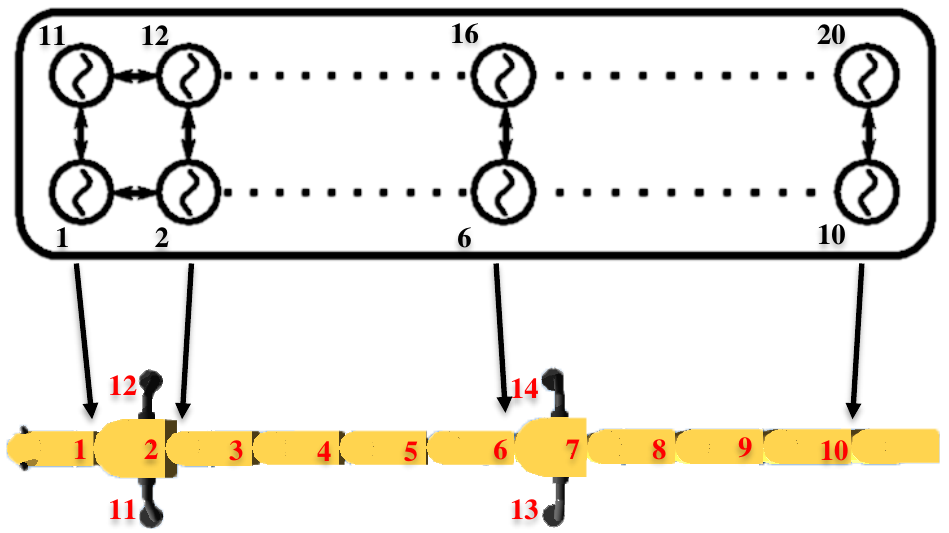
\includegraphics[width=0.5\textwidth]{figures/model_controller.png}
  \caption[Controller model]{A double chain of oscillators controlling
    the robot’s spine.}
  \label{fig:controller-model}
\end{figure}

\begin{figure}[ht]
  \centering 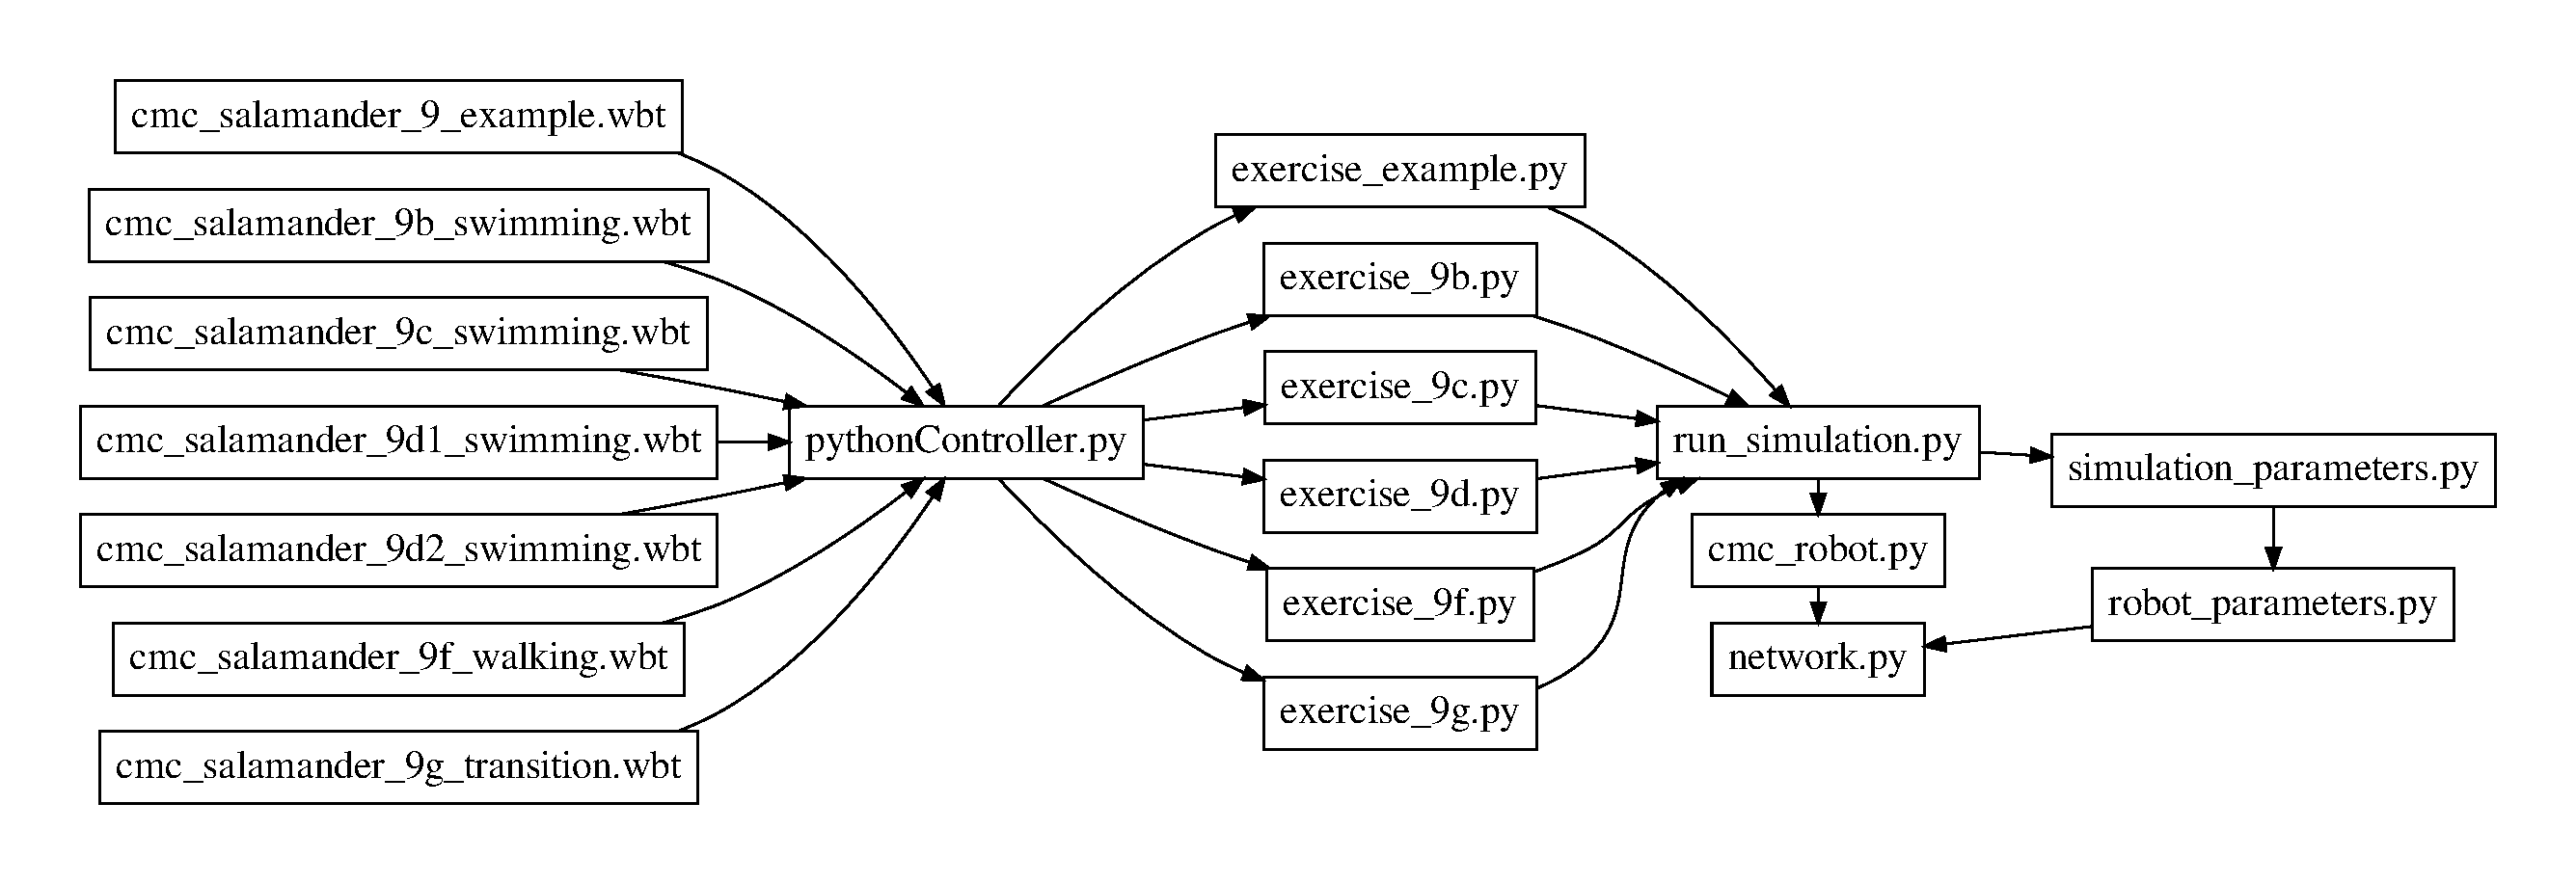
\includegraphics[width=1.0\textwidth]{figures/files}
  \caption{\label{fig:files} Exercise files dependencies. In this lab, you will
    be modifying \fileref{exercise1.py} and \fileref{pendulum\_system.py}}
\end{figure}

% \newpage

\subsection*{Code organization}
\label{subsec:code}

\begin{itemize}
\item \corr{\textbf{Webots::worlds::cmc\_salamander\_\#.wbt}} - These are the
  world files which describe the worlds and allow to run the simulations. You
  can run a simulation by running this file with Webots. It also automatically
  loads the pythonController. Note that each of these files will also run the
  appropriate \corr{exercise\_\#.py} such that you can run each exercise
  separately. Note that the simulation of the exercises may close immediately as
  they are not implemented yet. Only \corr{cmc\_salamander\_9\_example.wbt} will
  run for a few seconds before closing.
\item \corr{\textbf{Webots::controllers::pythonController::exercise\_\#.py}} -
  To be used to implement and answer the respective exercise questions. Note
  that \corr{exercise\_example.py} is provided as an example to show how to run
  a parameter sweep. Note that network parameters can be provided here.
\item \corr{\textbf{Webots::controllers::pythonController::pythonController.py}}
  - The main robot controller is implemented in pythonController.py. This file
  is the main file called by Webots during simulations and can call classes and
  functions from other files to control the robot and log data. This file is
  mainly used for calling the appropriate \corr{exercise\_\#.py} file. Note that
  by default the simulation will close Webots when it finishes. If you do not
  want Webots to close, you can comment the following line:
  \texttt{world.simulationQuit(0)}.
\item \corr{\textbf{Webots::controllers::pythonController::run\_simulations.py}}
  There is a run\_simulation.py function which is provided for convenience
  to easily run multiple simulations with different parameters. You are free to
  implement other functions to run simulations as necessary.
\item \corr{\textbf{Webots::controllers::pythonController::cmc\_robot.py}} -
  Contains the SalamanderCMC class, which is used for controlling and logging
  the robot.
\item
  \corr{\textbf{Webots::controllers::pythonController::experiment\_logger.py}} -
  Contains the codes for logging the simulation. Feel free to modify this file
  to extend the logging capabilities. Note that the logging makes use of
  Numpy.savez to save the data.
\item \corr{\textbf{Webots::controllers::pythonController::network.py}} - This
  file contains the different classes and functions for the CPG network and the
  Ordinary Differential Equations (ODEs). You can implement the network
  parameters and the ODEs here. Note that some parameters can be obtained from
  pythonController.py to help you control the values.
\item
  \corr{\textbf{Webots::controllers::pythonController::robot\_parameters.py}} -
  This file contains the different classes and functions for the parameters of
  the robot, including the CPG network parameters. You can implement the network
  parameters here. Note that some parameters can be obtained from
  SimulationParameters class in \corr{simulation\_parameters.py} and sent by
  \corr{exercise\_\#.py} to help you control the values (refer to example).
\item
  \corr{\textbf{Webots::controllers::pythonController::simulation\_parameters.py}}
  - This file contains the SimulationParameters class and is provided for
  convenience to send parameters to the setup of the network parameters in
  \corr{robot\_parameters.py}. All the values provided in SimulationParameters
  are actually logged in \corr{cmc\_robot.py}, so you can also reload these
  parameters when analyzing the results of a simulation.
\item \corr{\textbf{Webots::controllers::pythonController::solvers.py}} - This
  features fixed time-step solvers which will can are used by network.py for
  solving the ODE at each time-step. Feel free to switch between the Euler and
  the Runge-Kutta methods. \textit{You do not need to modify this files.}
\item \corr{\textbf{Webots::controllers::pythonController::run\_network.py}} -
  By running the script from Python, Webots will be bypassed and you will run
  the network without a physics simulation. Make sure to use this file for
  question 9a to help you with setting up the CPG network equations and
  parameters and to analyze its behavior. This is useful for debugging purposes
  and rapid controller development since starting the Webots simulation with
  physics takes more time.
\item \corr{\textbf{Webots::controllers::pythonController::plot\_results.py}} -
  Use this file to load and plot the results from the simulation. This code runs
  with the original pythonController provided.
\item \corr{\textbf{Webots::controllers::pythonController::parse\_args.py}} -
  Used to parse command line arguments for run\_network.py and plot\_results.py
  and determine if plots should be shown or saved directly. \textit{You do not
    need to modify this files.}
\item \corr{\textbf{Webots::controllers::pythonController::save\_figures.py}} -
  Contains the functions to automatically detect and save figures. \textit{You
    do not need to modify this files.}
\item
  \corr{\textbf{Webots::controllers::pythonController::exercise\_example.py}} -
  Contains the example code structure to help you familiarize with the other
  exercises. \textit{You do not need to modify this files.}
\end{itemize}

% \newpage

\section*{Prerequisites}

\subsection*{Make sure you have successfully installed Webots by
  following the instructions outlined in Lab 7}

\subsection*{Complete the tutorial and practice examples of Webots as
  outlined in Lab 7}

\subsection*{Open the \fileref{Webots::worlds::cmc\_salamander\_9\_example.wbt} file
  in Webots. This should launch the Salamandra robotica model in
  simulation world}

\subsection*{Running the simulation}
Now when you run the simulation, the Salamandra robotica model should
float on the water with no errors in the Webots console dialog. At
this point you can now start to work on implementing your exercises.

\newpage

\section*{Questions}

The exercises are organized such that you will have to first implement the
oscillator network model in \corr{run\_network.py} code and analyze it before
connecting it to the body in the Webots world.  Exercise 9a describes the
questions needed to implement the oscillator models. After completing exercise
9a you should have an oscillator network including both the spinal CPG and limb
CPG.

Using the network implemented in exercise 9a you can explore the swimming,
walking and transition behaviors in the Salamandra robotica model using Webots
and complete the exercises 9b to 9g.

\subsection*{9a. Implement a double chain of oscillators along with
  limb CPG's}
\label{sec:implement-chain}

Salamandra robotica has 10 joints along its spine and 1 joint for each
limb. The controller

\begin{equation}
  \label{eq:dphase}
  \dot{\theta}_i = 2 \pi f + \sum_j r_j w_{ij} sin(\theta_j - \theta_i - \phi_{ij})
\end{equation}

\begin{equation}
  \label{eq:dr}
  \dot{r}_i = a (R_i - r_i)
\end{equation}

\begin{equation}
  \label{eq:output}
  \dot{q}_i = r_i(1 + cos(\theta_i)) - r_{i+10}(1 + cos(\theta_{i+10})) \text{ if body joint}
\end{equation}

with $ \theta_i $ the oscillator phase, f the frequency, $ w{_ij} $ the coupling
weights, $ \phi_{ij} $ the nominal phase lag (phase bias), $ r_i $ the
oscillator amplitude, $ R_i $ the nominal amplitude, $ a $ the convergence
factor and $ q_i $ the spinal joint angles.


\begin{enumerate}
\item Implement the double chain oscillator model using the functions
  \fileref{network.py::network\_ode}. Test your implementation by running the
  network using \fileref{run\_network.py}. For the network parameters check
  lecture slides (pay attention to different number of segments). You can also
  find more information in \cite{ijspeert2007swimming} (especially in the
  supplementary material). You can set all the network parameters in the
  \fileref{robot\_parameters.py::RobotParameters}. To facilitate your work, you
  could start by only implementing the network for the body oscillators
  ($i=[0, ..., 19]$) and ignoring the leg oscillators ($i=[20, ..., 23]$). Refer
  to \corr{network::RobotState} and
  \corr{robot\_parameters.py::}\-\corr{RobotParameters} for the dimensions of
  the state and the network parameters respectively.

\item Implement the output of your CPG network to generate the spinal joint
  angles according to equation \ref{eq:output}. Implement this in the function
  \fileref{network.py::motor\_output}. Verify your implementation in by running
  the Python file \fileref{run\_network.py}.  Use the functions in
  \fileref{plot\_results.py} to report your spinal joint angles $q_i$.

\item Implement a drive and show that your network can generate swimming and
  walking patterns similarly to \cite{ijspeert2007swimming}.


  \textbf{Hint:} The state for the network ODE is of size 48 where the first 24
  elements correspond to the oscillator phases $\theta_i$ of the oscillators and
  the last 24 elements correspond to the amplitude $r_i$. The initial state is
  set in the init of \corr{network.py::SalamanderNetwork}.
\end{enumerate}

\paragraph{Answer}

By using the function 'run\_network.py', we were able to test our parameters and obtain the following behavior for the walking and swimming pattern:

\paragraph{Swimming (drive = 4)}

By choosing a drive of 4, the robot adopt a swimming behavior. In this configuration, the legs are not moving as we can see in Figure \ref{fig_ampli_4} where the amplitude of the legs in red is equal to zero. Also, the amplitude of the oscillations of the spinal joints is quite high with a high frequency of oscillations to be able to go through an aqueous medium as can be seen in Figure \ref{fig_spinal_4}

\begin{minipage}[c]{.48\linewidth}
\begin{figure}[H]
    \centering
    \includegraphics[width = 0.9\linewidth]{9a/Spinal_joint_angle_with_a_drive_of_4dot0.pdf}
    \caption{Spinal joint angle with a drive of 4}
    \label{fig_spinal_4}
\end{figure}

\end{minipage}
\hfill
\begin{minipage}[c]{.48\linewidth}
\begin{figure}[H]
    \centering
    \includegraphics[width = 0.9\linewidth]{9a/Amplitude_of_the_joints_with_a_drive_of_4dot0.pdf}
    \caption{Amplitude of the joints for a drive of 4}
    \label{fig_ampli_4}
\end{figure}

\end{minipage}

\paragraph{Walking (drive = 2)}

By choosing a drive of 2, the robot adopts a walking behavior. In this configuration, the legs are moving as we can see on Figure \ref{fig_ampli_2} where the amplitude of the legs in red is not zero anymore. Also, the amplitude of the joints is lower this time and oscillate with a slower frequency as can be seen on figure \ref{fig_spinal_2}. This is usual for the walking pattern were the robot becomes slower and does not rely anymore on a high oscillation to move itself.

\begin{minipage}[c]{.48\linewidth}
\begin{figure}[H]
    \centering
    \includegraphics[width = 0.9\linewidth]{9a/Spinal_joint_angle_with_a_drive_of_2dot0.pdf}
    \caption{Spinal joint angle with a drive of 2}
    \label{fig_spinal_2}
\end{figure}

\end{minipage}
\hfill
\begin{minipage}[c]{.48\linewidth}
\begin{figure}[H]
    \centering
    \includegraphics[width = 0.9\linewidth]{9a/Amplitude_of_the_joints_with_a_drive_of_2dot0.pdf}
    \caption{Amplitude of the joints for a drive of 2}
    \label{fig_ampli_2}
\end{figure}

\end{minipage}



\subsection*{9b. Effects of amplitude and phase lags on swimming
  performance}
\label{sec:amplitude-phase-performance}

Now that you have implemented the controller, it is time to run experiments to
study its behaviour. How does phase lag and oscillation amplitude influence the
speed and energy? Use the provided \corr{run\_simulation.py::run\_simulation()}
to run a grid search to explore the robot behavior for different combinations of
amplitudes and phase lags. Use \corr{plot\_results.py} to load and plot the
logged data from the simulation. Feel free to extend the logging in
\corr{cmc\_robot.py} to show additional measurements if necessary. Include 2D/3D
plots showing your grid search results and discuss them. How do your findings
compare to the wavelengths observed in the salamander?

% Run the grid search twice, for frequencies of 1Hz and 2Hz.

\begin{itemize}
\item \textbf{Hint 1:} To use the grid search, check out the function
  \corr{run\_simulation.py::run\_simulation()} and the example provided in
  \corr{exercise\_example.py}. This function takes the desired parameters as a
  list of SimulationParameters objects (found in
  \corr{simulation\_parameters.py}) and runs the simulation. Note that the
  results are logged as simulation\_\#.npz in a specified log folder. After the
  grid search finishes, the simulation will close, you can remove this feature
  by commenting world.simulationQuit(0) in \corr{pythonController.py::main()}.
\item \textbf{Hint 2:} An example how to load and visualise grid
  search results is already implemented in
  \corr{plot\_results.py::main()}. Pay attention to the name of the
  folder and the log files you are loading. Before starting a new grid
  search, change the name of the logs destination folder where the
  results will be stored. In case a grid search failed, it may be
  safer to delete the previous logs to avoid influencing new results
  by mistake.
\item \textbf{Hint 3:} Estimate how long it will take to finish the
  grid search. Our suggestion is to choose wisely lower and upper
  limits of parameter vectors and choose a reasonable number of
  samples. To speed-up a simulation, make sure to run Webots in a fast
  mode.
\item \textbf{Hint 4:} Energy can be estimated by integrating the
  product of instantaneous joint velocities and torques. Feel free to
  propose your own energy metrics, just make sure to include the
  justification.
\end{itemize}

\subsection*{Answer}

\begin{figure}[H]
 
\begin{subfigure}{0.5\textwidth}
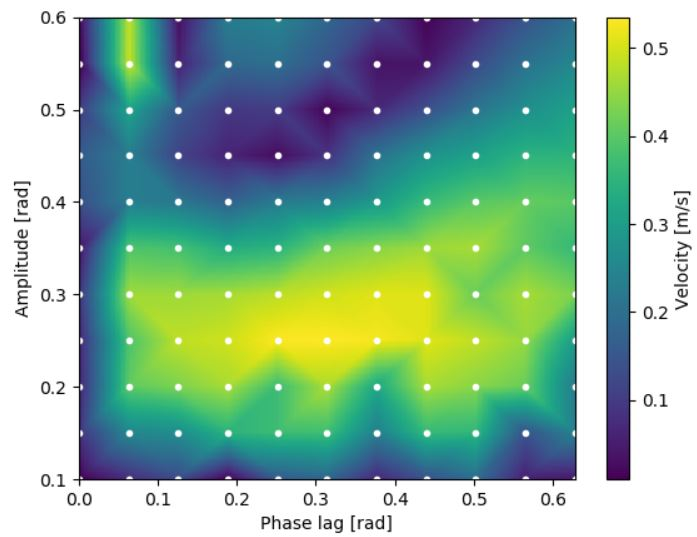
\includegraphics[width=8cm]{9b_vel.JPG}
\caption{Velocity}
\label{fig:9b1}
\end{subfigure}
\begin{subfigure}{0.5\textwidth}
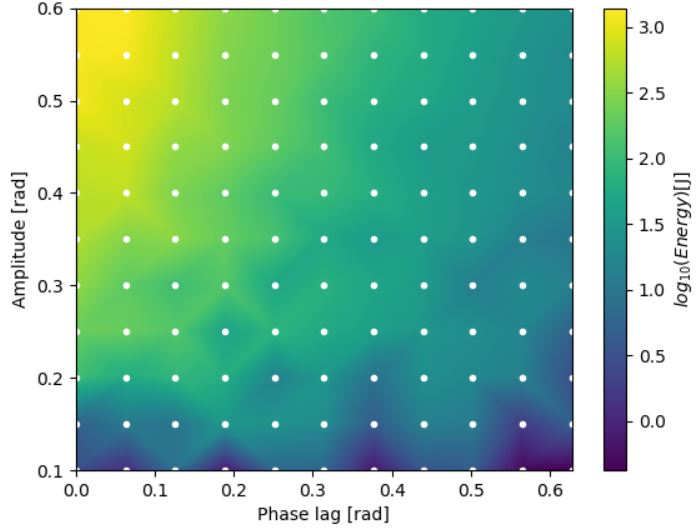
\includegraphics[width=8cm]{9b_en.JPG}
\caption{Energy}
\label{fig:9b2}
\end{subfigure}
 
\caption{Velocity and Energy with varying amplitude and phase lag}
\label{fig:9b}
\end{figure}

The oscillator synchronizes at the fixed point $$ \rho_{\infty}= arcsin(A) + \phi_{12} $$
$$A=\frac{2\pi(v_2-v_1)}{R_2w_{12}}$$

This equation has no solution if A>1, one solution if A=1 and two solution if A<1. If A<1 the stability is defined by the sign of the function below. The fixed point is stable if this quantity is negative, and unstable if it is positive.
$$\mbox{If A=1 }  \rho_{\infty}=\pm \frac{\pi}{2}+\phi_{12}$$
$$\mbox{If A<1 Sign Function : }  R_{2}w_{12}cos(\rho_{\infty}-\phi_{12})$$

From those equation we see that if we decrease the amplitude too much the factor A will increase above and hence the oscillator will drift. 
In the case of the phase lag, this value will only influence the stability through the equation above. 

We run this grid search with a drive of 4.0, amplitudes varying from 0.1 to 0.6 and phase lag varying from 0 to $\frac{\pi}{5} $. Higher phase lags caused the salamander to either fold on itself, oscillate along the spine without moving, move backwards or oscillate between forward and backward motion, all of which falsify our results. The velocity is calculated as the distance travelled over time, starting 4 seconds after the start of the simulation in order to compare the stable speed of each pair of parameter and avoid the initial acceleration that could falsify results.

In Figure \ref{fig:9b2} we can see a spike of energy for maximum amplitude and low phase lag, with the energy lowering as the amplitude decreases and the phase lag increases. This makes sense since higher amplitudes will require an higher amount of energy to move the salamander. We can also see that this region does not correspond to a high velocity, which means the salamander spends a lot of energy moving around and turning on itself without actually moving forward. This is due to this high amplitudes which make the robot turn too much at each oscillation. This means that a non negligible part of the energy of the robot is lost in an oscillating behavior which is not contributing to the movement.

An aberration of the simulation can be seen for an amplitude of 0.55 and a phase lag of $\frac{\pi}{5} $ where the salamander curls completely on itself on one side then on the next one. It expands tremendous amounts of energy in doing so but manages to move quite fast, albeit completely unnaturally. This type of behavior can be observed in simulation but would be both dangerous and unnecessary in real life since better speeds can be reached with much less effort.

As we can see in Figure \ref{fig:9b1}, the velocity is optimal for an amplitude of around 0.25 and a phase lag of around 0.32. Various combinations of phase lag and amplitudes around those values also work well as it approaches optimal velocity. We can also see that with a phase lag of 0 the salamander is almost unable to move due to have no oscillation that spread throughout its body without creating an united movement. It has the same behavior as mentioned previously, curling up in a circle on one side then the other, once again expanding a lot of energy for little forward motion.


Optimal behavior would be fast movement with minimal energy and this can be found in the same zone as mentioned previously. We can note that coordinates with higher velocity correspond to the coordinates with a higher energy since more energy is required to move faster. However with good calibrations of both parameters, high velocity can be reached with relatively low energy since the robot will reach a stable behavior where most of its energy is spent moving forward instead of to the sides. These values induce a very smooth movement that makes the salamander move fast at a low energy cost.



\subsection*{9c. Amplitude gradient}
\label{sec:amplitude-gradient}

\begin{enumerate}
\item So far we considered constant undulation amplitudes along the body for
  swimming. Implement a linear distribution of amplitudes along the spine,
  parametrized with two parameters: amplitudes of the first (Rhead) and last
  (Rtail) oscillator in the spine (corresponding to the first and last
  motor). To do so, you can add a parameter amplitudes=[Rhead, Rtail] in
  \corr{simulation\_parameters.py::SimulationParameters}. Don't forget to modify
  \corr{robot\_parameters.py::}\-\corr{RobotParameters::set\_nominal\_amplitudes()}
  and interpolate the amplitude gradient between values Rhead and Rtail within
  the function. Note that you can then provide this amplitudes parameter from
  \corr{exercise\_9b.py}.
\item Run a grid search over different values of parameters Rhead and
  Rtail (use the same range for both parameters). How does the
  amplitude gradient influence swimming performance (speed, energy)?
  Include 3D plots showing your grid search results. Do it once, for
  frequency 1Hz and total phase lag of $2\pi$ along the spine.
  

  
\item How is the salamander moving (with respect to different body
  amplitudes)?  How do your findings in 2) compare to body
  deformations in the salamander?  Based on your explorations, what
  could be possible explanations why the salamander moves the way it
  does?
\end{enumerate}

\subsection*{Answer}

\textbf{2.} 
\begin{figure}[H]

\begin{subfigure}{0.5\textwidth}
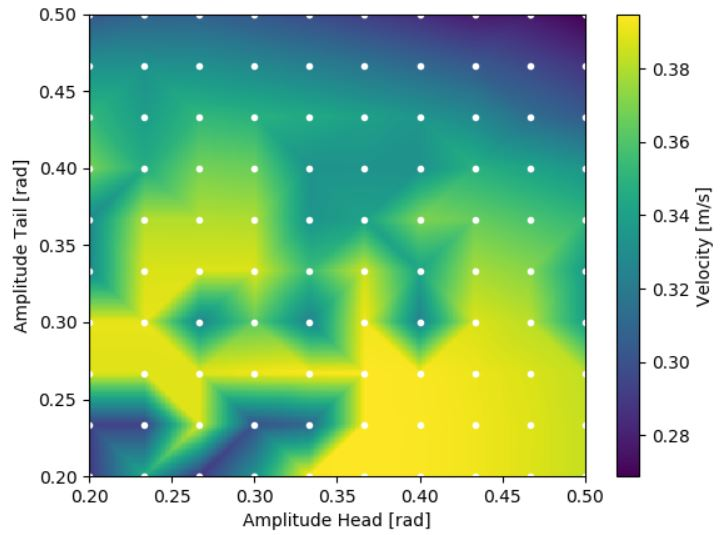
\includegraphics[width=8cm]{9c_vel.JPG}
\caption{Velocity}
\label{fig:9c1}
\end{subfigure}
\begin{subfigure}{0.5\textwidth}
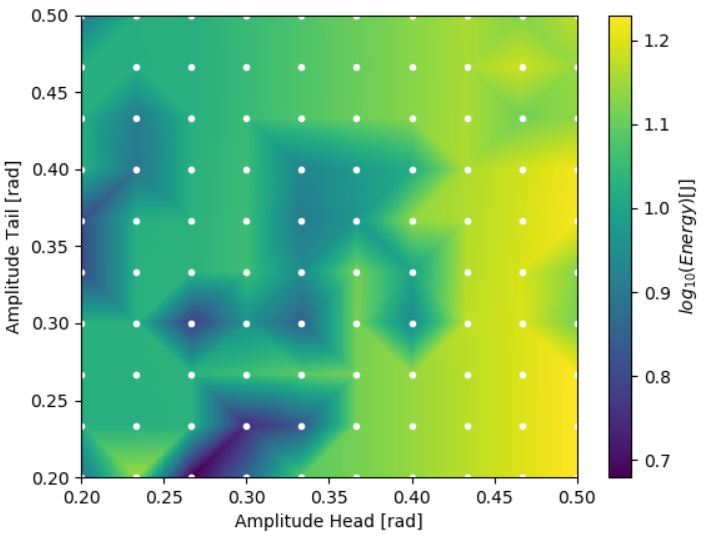
\includegraphics[width=8cm]{9c_en.JPG}
\caption{Energy}
\label{fig:9c2}
\end{subfigure}

\begin{center}
\begin{subfigure}{0.5\textwidth}
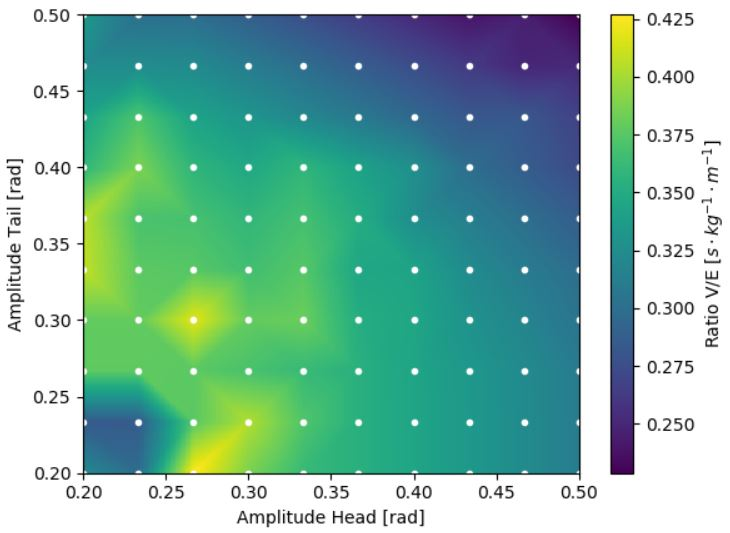
\includegraphics[width=8cm]{9c_ratio.JPG}
\caption{Ratio}
\label{fig:9c3}
\end{subfigure}    
\end{center}

 
\caption{Velocity and Energy with amplitude gradient}
\label{fig:9c}
\end{figure}

We ran the grid search for amplitudes varying from 0.2 to 0.5 since higher amplitudes caused saturation and lower amplitudes are not sufficient to make the robot move properly when the phase lag is 0, as can be seen in \ref{fig:9b1}.

We can see the influence of different amplitudes gradients on velocity and energy in Figure \ref{fig:9c}. First of all we can see a clear correlation between the velocity reached and the energy expended which is logical since lower velocities required less energy. We also see a general trend in both graphs. In Figure \ref{fig:9c1} we see that velocity increases as the tail amplitude decreases. This corresponds with results from 9b where amplitudes that are too high make the salamander curve too much and move more perpendicularly than forward. In Figure \ref{fig:9c2} we see that the energy increases with both amplitudes, but mainly the head amplitude. When the head amplitude is high, the movement starts at the head and the rest of the body follows, which means the salamander has to pull the rest of its body which works well but requires a lot of energy. When the head amplitude is smaller, the movement starts lower in the body and the salamander uses its spine to push itself forward, which takes longer to accelerate but requires less energy.

Optimal behavior is a high velocity for a low energy, and when we look at the graphs we can see several combinations of amplitudes where the velocity and energy are lower. However the velocity is only slightly lower than the maximal where as the energy is much lower since it is on a logarithmic scale. We computed a ratio of velocity over energy to find the optimal behavior which can be seen in Figure \ref{fig:9c3}. We found was that optimal behavior prioritize low energy even if the velocity suffers slightly. This makes sense since the decreases of velocity is much smaller than the one of the energy which means that the relation between the two seems linear but with a slope lower than 1 : a lot of energy is necessary for a small increase in speed. Therefore, gaits with low energy should be prioritized since they are close in speed to more costly gaits but require very little energy. 

Although those gaits are not the fastest, they are the one let the salamander escape its static position the most easily by generating the smoothest movements.



\textbf{3.} The salamander moves forward but with obvious different amplitudes along the spine. Higher amplitudes makes the movements more sinuous so that the salamander travels more distance without actually getting much further from its original point. Basically, the optimal behavior is the one that is most fluid and harmonious and can be reached through several combinations.

As mentioned above, with a higher amplitude in the tail, the salamander pushes forward using its body, whereas when the amplitude is higher in the head than in the tail, it must pull its body using its head, which requires a lot more energy. 

\subsection*{9d. Turning and backwards swimming}
\label{sec:turning-backwards}

\begin{enumerate}
\item How do you need to modulate the CPG network (\corr{network.py})
  in order to induce turning?  Implement this in the Webots model and
  plot example GPS trajectories and spine angles.
  
\begin{figure}[H]

\begin{subfigure}{0.5\textwidth}
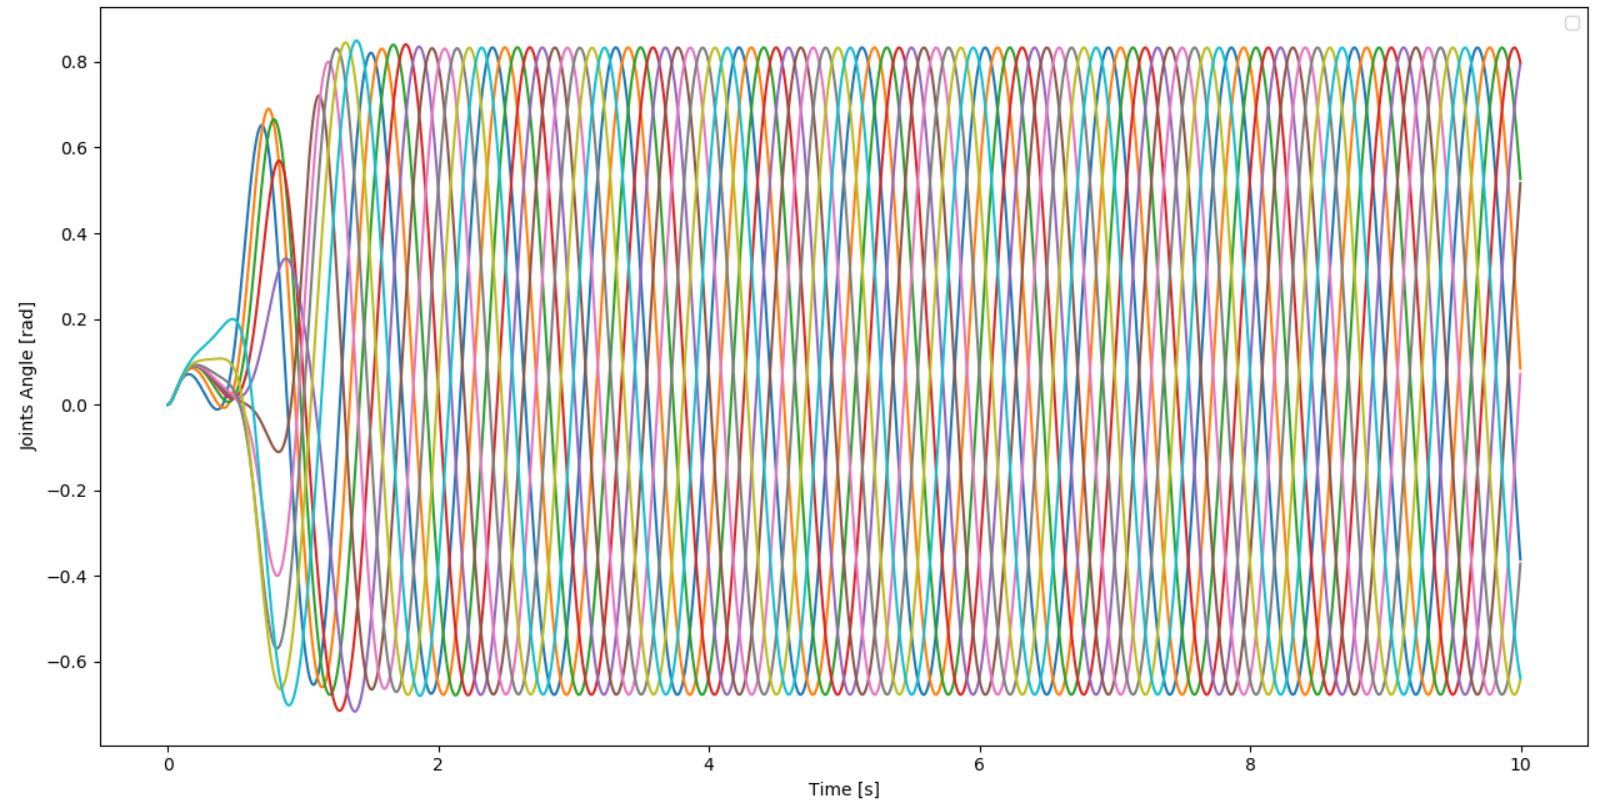
\includegraphics[width=16cm]{9d1_pos.JPG}
\begin{center}
\caption{Joints Angles when turning}
\end{center}    
\label{fig:2_a_1}
\end{subfigure}    

\begin{center}
\begin{subfigure}{0.5\textwidth}
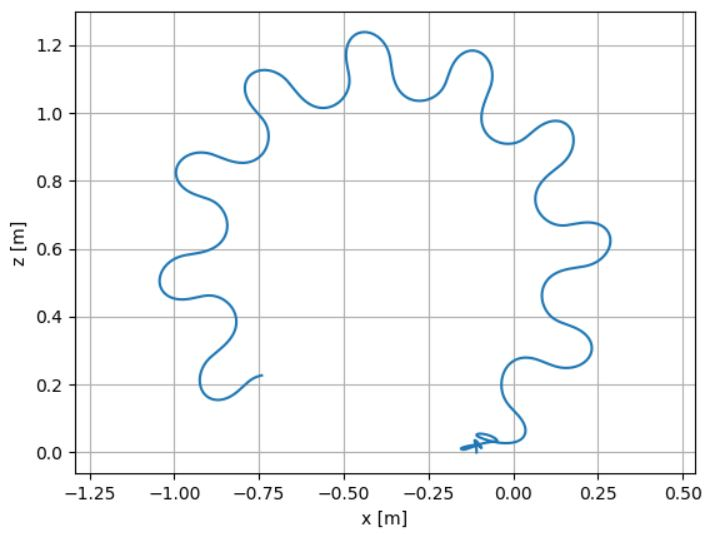
\includegraphics[width=8cm]{9d1_traj.JPG}
\caption{Trajectory}
\label{fig:2_a_2}
\end{subfigure}
 \end{center}
\caption{Position and Trajectory when turning}
\label{fig:9d1}
\end{figure}


\hspace{6mm}
To induce turning, we set a different drive for the two sides of the body for the setting of the nominal amplitude only. One side has a higher drive and hence produces a higher amplitude while the side with a lower drive has a smaller amplitude.  The salamander will then turn to the side with the lowest amplitude. The difference in amplitude is determined by the value of the turn we wish to induce, the higher the value, the more the robot will turn. We used a turn value of 0.15 with a drive of 4.0 for Figure \ref{fig:9d1}.\\
This configuration will induce a drive of 4.6($= 4\cross(1+0.15)$) on the left side and a drive of 0.6 ($= 4\cross0.15$) on the right side of the salamander. This behavior, hence induce a turning in the right direction (the graph below is a view from the bottom of the robot hence theapparentt turning in the left direction). 
  
  
\item How could you let the robot swim backwards? Explain and plot
  example GPS trajectories and spine angles.
\end{enumerate}

\begin{figure}[H]
\centering
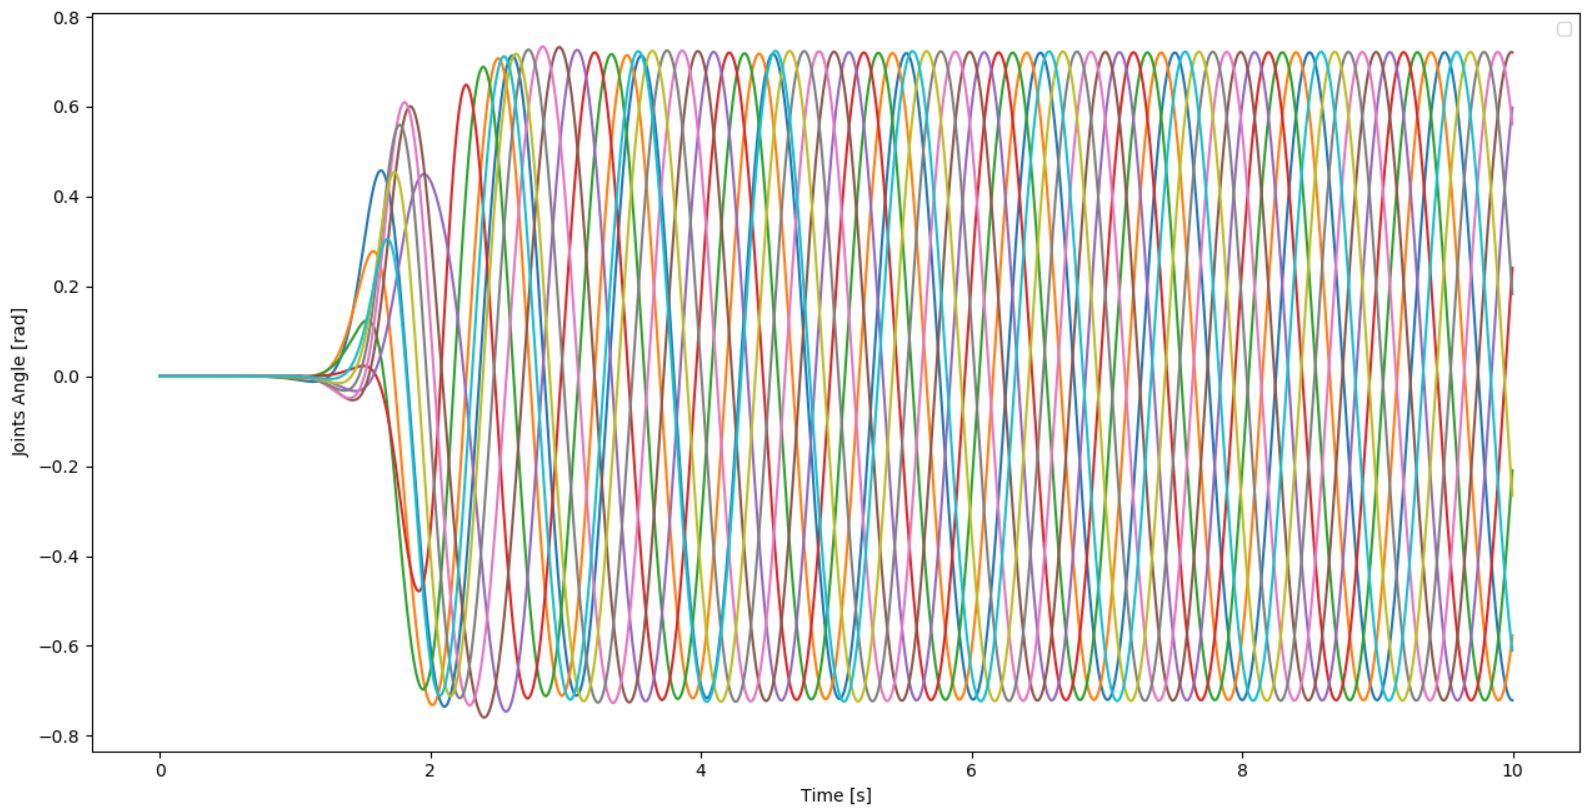
\includegraphics[width=16cm]{9d2_pos.JPG}
\caption{Joints Angles when going backward}
\centering
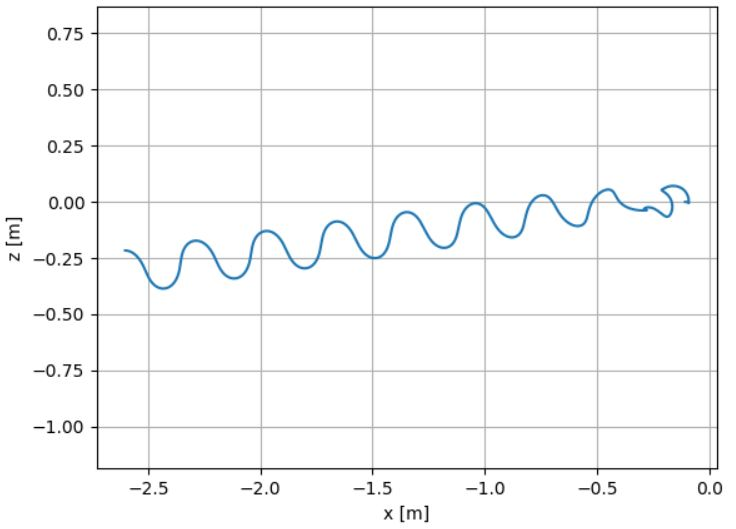
\includegraphics[width=8cm]{9d2_traj.JPG}
\caption{Trajectory when going backward}


\label{fig:9d2}
\end{figure}

%The model shows that changing the intrinsic frequency of some oscillators leads to changes in the phase lags. This can be the mechanism for backward swimming. By stimulating more the oscillators at the tail (i.e. by increasing their intrinsic frequency), this could possibly lead to a reversal of the traveling wave. 
 
\hspace{6mm}The robot moves by setting a different phase bias throughout its body so that each joints moves one after the other and not all in the same direction at once. To move backwards, we simply need to input the opposite phase bias to inverse the oscillation movement so that the tail starts the movement instead of the head. This way, instead of pushing with its tail to move forward, the salamander pushes with its head to move backwards. We used a drive of 3.5 for Figure \ref{fig:9d2}.


\subsection*{9e. Cancelled}

\subsection*{9f. Limb – Spine coordination}
\label{sec:limb-spine-coordination}

In this next part you will explore the importance of a proper coordination
between the spine and the limb movement for walking.

\begin{enumerate}
\item Change the drive to a value used for walking and verify that the robot
  walks
\item Analyze the spine movement: What are your phase lags along the spine
  during walking? How does the spine movement compare to the one used for
  swimming?

  
\item Notice that the phase between limb and spine oscillators affects the
  robot’s walking speed. Run a parameter search on the phase offset between
  limbs and spine. Set the nominal radius R to 0.3 [rad]. Include plots showing
  how the phase offset influences walking speed and comment the results. How do
  your findings compare to body deformations in the salamander while walking?
 

\item Explore the influence of the oscillation amplitude along the body with
  respect to the walking speed of the robot. Run a parameter search on the
  nominal radius R with a fixed phase offset between limbs and the spine. For
  the phase offset take the optimal value from the previous sub-exercise. While
  exploring R, start from 0 (no body bending).
\end{enumerate}

Include plots showing how the oscillation radius influences walking speed and
comment on the results.



\subsection*{Answer}


\textbf{2.} The phase lag along the spine are set to 0 for a walking behavior. This is because since the legs are making the body move there is no need for a phase lag along the spine to create a movement. This means the whole body moves at the same time in a sinuous manner and uses only the support of the legs to move forward. \\

\textbf{3.}  
\begin{figure}[H]
\centering
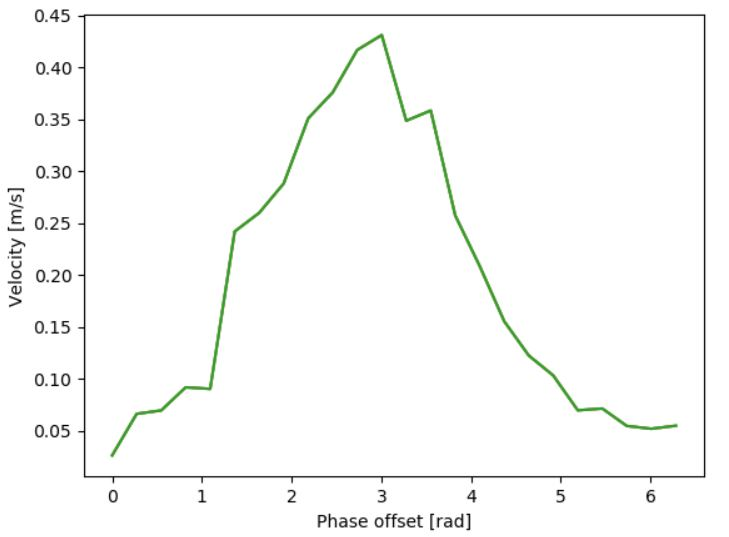
\includegraphics[scale=0.7]{9f_3.JPG}
\caption{Walking speed depending on phase offset}
\label{fig:9f3}
\end{figure}

We ran an experiment testing the robot's walking speed for a phase offset between spine and leg varying between $0$ and $2\pi$. We can see the speed has maximum around $pi$. This is because it is the phase offset between legs and spine which correspond to a synchronous movement between the two. The spine and the legs moves together, facilitating movement and increasing the walking speed. \\

\newpage
\textbf{4.} 
\begin{figure}[H]
\centering
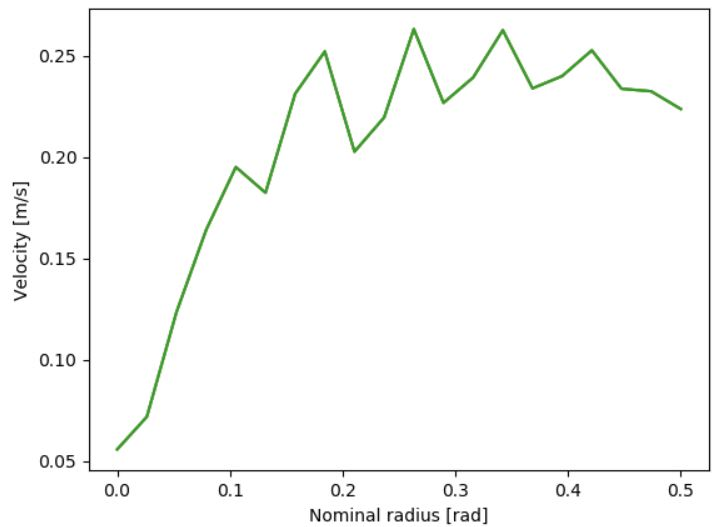
\includegraphics[scale=0.5]{9f_4.JPG}
\caption{Walking speed depending on Nominal radius}
\label{fig:9f4}
\end{figure}

We ran the experiment to see the influence of the oscillation amplitude on the walking speed. We tested with a drive of 1.5 for amplitudes between 0 and 0.5 since anything higher caused saturation or abnormal behavior. We use $\pi$ for the phase offset value since it is the optimal value.

We can see from Figure \ref{fig:9f4} that the salamander requires a minimal nominal radius of around 0.1 to move properly. When there is too little bending, the salamander's legs are asynchronous with its body so much that it spends most of the simulation on its belly with its legs moving around above its body.

We can see that some values for nominal radius allow for a faster walking speed. This is once again due to synchronization between the legs and the body, this time reached through the amplitude of the body. The body moves in a way so that each foot is set down when the leg is facing forward, then the body rotates around the leg to move the opposite leg forward. The back legs move in opposite to the front leg, meaning that when the front left foot is down, the back right foot is also down. This gait uses the sinuous movement of the spine to optimize the speed of the walking salamander. Some amplitudes work better than others with the maximal velocity being reached when the front and back legs are in perfect opposite synchronisation, with for example the front right foot and back left foot being set down at the exact same time. Lower velocities are due to the salamander front and back legs being slightly asynchronous.



\subsection*{9g. Land-to-water transitions}

\begin{enumerate}
\item In this exercise you will explore the gait switching mechanism. The gait
  switching is generated by a high level drive signal which interacts with the
  saturation functions that you should have implemented in 9a. Implement a new
  experiment which uses the x-coordinate of the robot in the world retrieved
  from a GPS reading (See \texttt{self.gps.getValues()} in
  \corr{cmc\_robot::log\_iteration()} for an example). Based on the GPS reading,
  you should determine if the robot should walk (it’s on land) or swim (it
  reached water). Depending on the current position of the robot, you should
  modify the drive such that it switches gait appropriately.
\item Run the Webots simulation and report spine and limb angles, together with
  the x coordinate from the GPS signal. Record a video showing the transition
  from land to water and submit the video together with this report.

\item (BONUS) Achieve water-to-land transition. Report spine and limb angles,
  the x-coordinate of the GPS and record a video.
\end{enumerate}


\textbf{Hint:} Use Webots’ internal video recording tool to easily record
videos.

\subsection*{Answer}

\textbf{2.}
\begin{figure}[H]
\centering

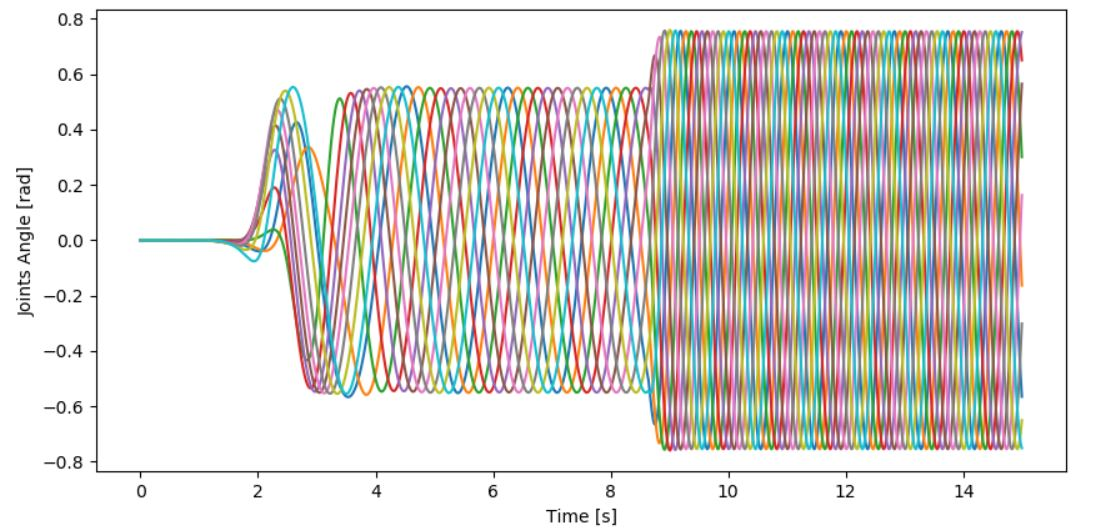
\includegraphics[width=16cm]{9g_joint.JPG}
\caption{Joints Angles when going from water to land}

\centering

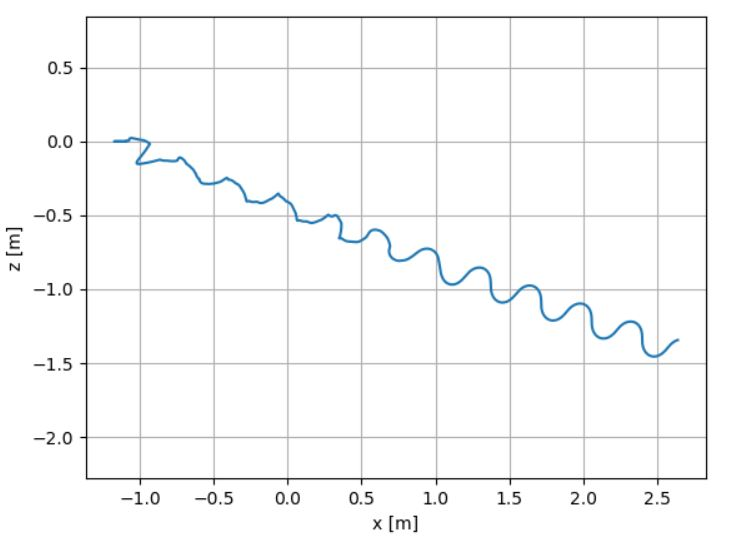
\includegraphics[width=8cm]{9g_gps.JPG}
\caption{Trajectory when going from water to land}

\label{fig:9g}
\end{figure}

The salamander starts with a drive of 1.5 for walking behavior and when it reaches the water it's drive is changed to 4.0 for a swimming behavior. 

The video of the salamander transitioning to the water can be found here : \href{https://drive.google.com/open?id=1XK0YEQ0OtI3paOIz72nGFJPvjhqrxoJy}{Transition Land to Water}\\

\newpage

\textbf{3.}
\begin{figure}[H]
\centering

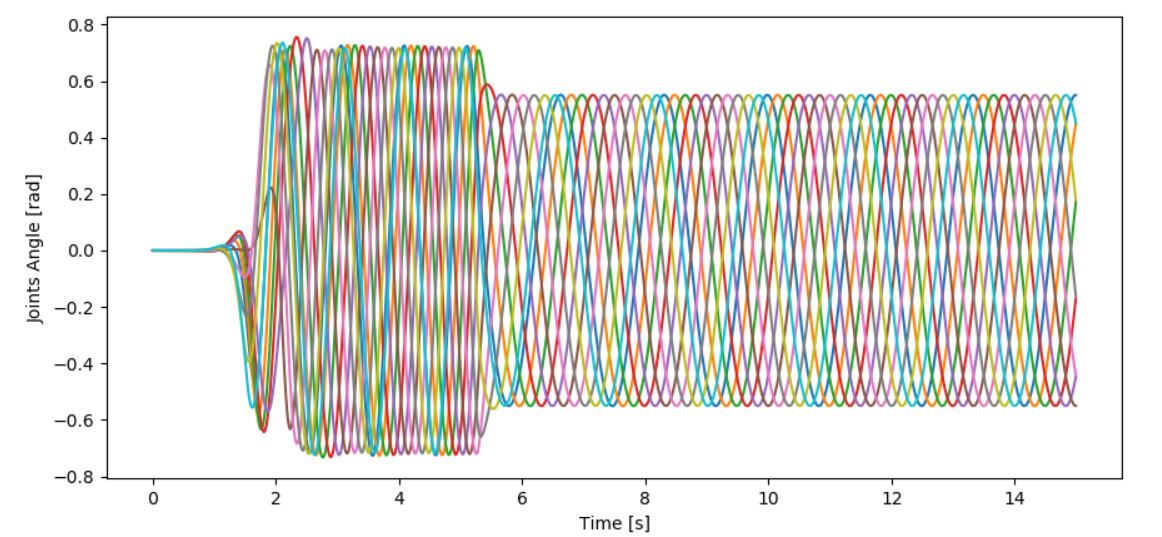
\includegraphics[width=16cm]{9g2_joints.JPG}
\caption{Joints Angles when going from land to water}

\centering

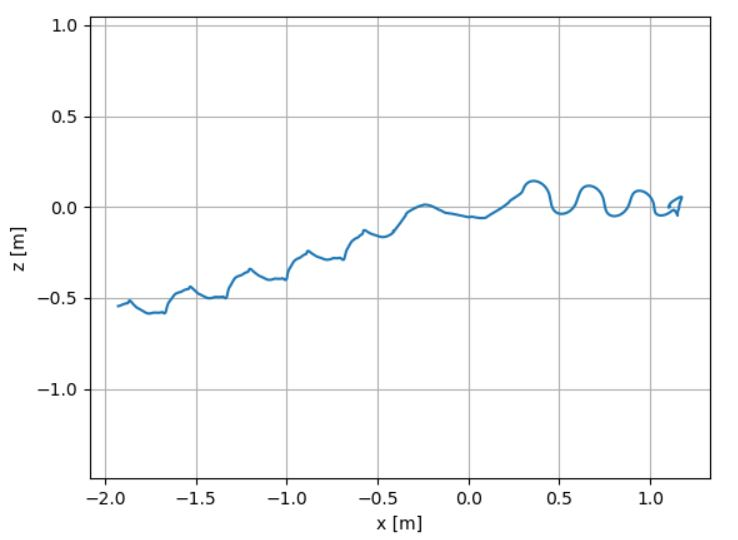
\includegraphics[width=8cm]{9g2_gps.JPG}
\caption{Trajectory when going from land to water}

\label{fig:9g2}
\end{figure}

The salamander starts with a drive of 4.0 for a swimming behavior and when it reaches the water it's drive is changed to 1.5 for walking behavior. 

The video of the salamander transitioning to land can be found here : \href{https://drive.google.com/open?id=1SsjYRnM28c-Y93Ew06Xjhznf4al96TmY}{Transition Water to Land}




\newpage

\bibliography{lab9}
\label{sec:references}
\bibliographystyle{ieeetr}


% \newpage

% \section*{APPENDIX}
% \label{sec:appendix}

\end{document}

%%% Local Variables:
%%% mode: latex
%%% TeX-master: t
%%% End: